%%% Содержимое слайдов

\frame[plain]{\titlepage} % Титульный слайд

%-------------------------------------------------------------------------------

\section{Станок Навигатор КС-12В}

\begin{frame}
\frametitle{\insertsection}


\begin{figure}
    \center
    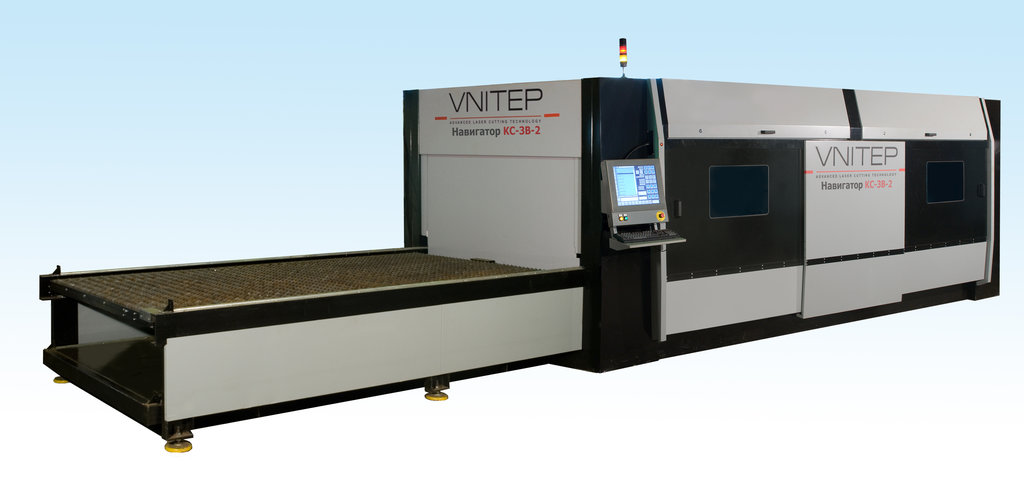
\includegraphics[width=4cm]{navigator.jpeg}
    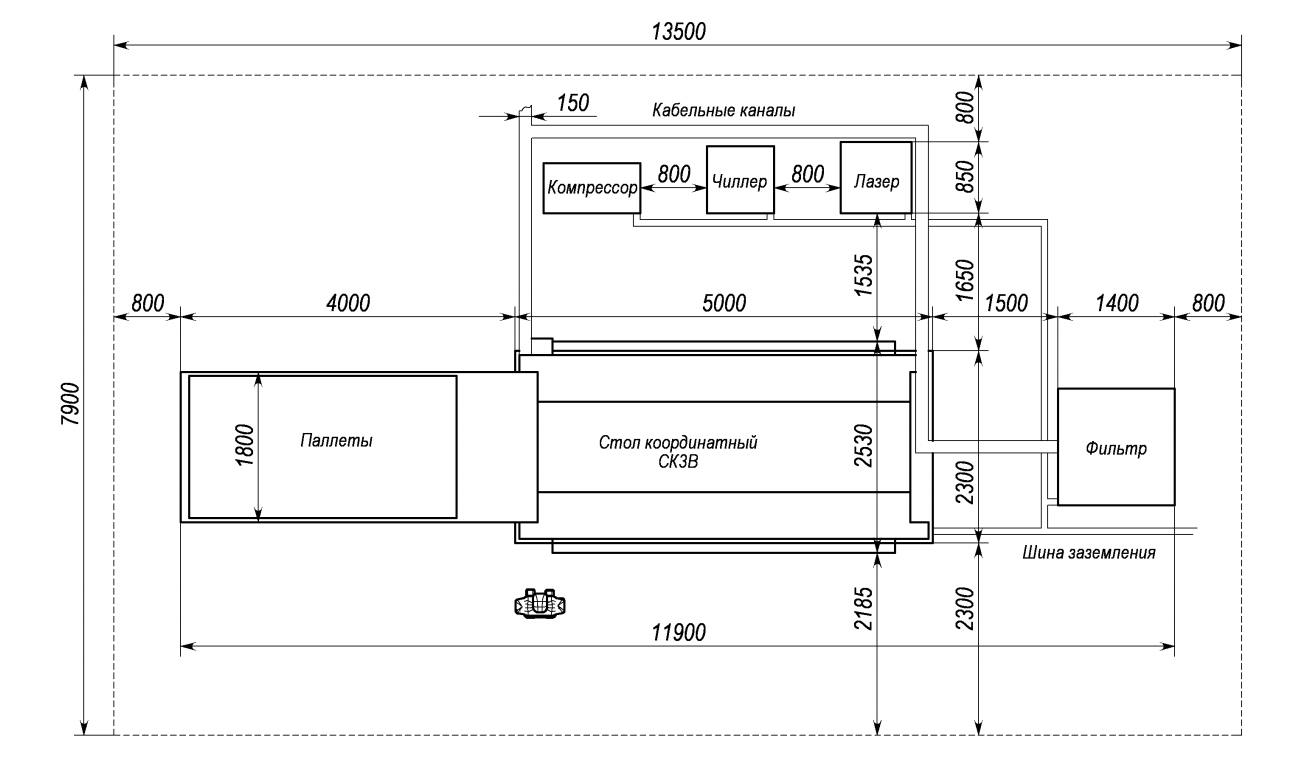
\includegraphics[width=5cm]{navigator.png}
\end{figure}

\begin{figure}
    \center
    
\includegraphics[width=2cm]{vnitep.png}
    
\includegraphics[width=2cm]{omnicube.png}
    
\includegraphics[width=2cm]{sespel.png}
\end{figure}

\end{frame}

%-------------------------------------------------------------------------------

\section{Актуальность}

\begin{frame}
\frametitle{\insertsection}

Актуальность работы обуславливается
отсутствием системы автоматического 
прогнозирования неисправностей для станков Навигатор.

\vspace{\baselineskip}

Кроме этого,
в целом существует область прогнозирования неисправностей
различных устройств. Данная область также является актуальной и быстроразвивающейся.

\end{frame}

%-------------------------------------------------------------------------------


\section{Цель}

\begin{frame}
\frametitle{\insertsection}

\textbf{Цель:} разработка системы для прогнозирования и обнаружения неисправностей
на станках лазерной резки Навигатор КС-12В компании ВНИТЭП

\vspace{\baselineskip}

\textbf{Объект:} станок лазерной резки Навигатор КС-12В.

\vspace{\baselineskip}

\textbf{Предмет:} система прогнозирования и обнаружения неисправностей для станка.

\end{frame}


%-------------------------------------------------------------------------------

\section{Задачи}

\begin{frame}
\frametitle{\insertsection}

\textbf{Задачи:}
\begin{itemize}
    \item анализ показателей и их краевых значений, предоставляющих сведения о неисправностях станка Навигатор;
    \item анализ существующих решений и подходов для прогнозирования неисправностей в устройствах;
    \item обработка и анализ накопленных данных со станка Навигатор;
    \item обоснование и выбор методов для прогнозирования и обнаружения неисправностей;
    \item разработка модели прогнозирования и программного модуля;
    \item введение разработанного модуля в эксплуатацию.
\end{itemize}

\end{frame}

%-------------------------------------------------------------------------------

\section{Существующие решения}

\begin{frame}
\frametitle{\insertsection}

\textbf{Неисправности:}
\begin{itemize}
    \item выход из строя лазерной головы станка;
    \item выход из строя оси XYZ;
    \item ошибки операторов.
\end{itemize}

\textbf{Существующие подходы к выявлению неисправностей:}
\begin{itemize}
    \item мониторинг ошибок оператором;
    \item мониторинг на основе показателей системы Omnicube;
    \item мониторинг программного обеспечения ЧПУ.
\end{itemize}


\end{frame}

%-------------------------------------------------------------------------------

\section{Мониторинг показателей и ошибок}

\begin{frame}
\frametitle{\insertsection}

\begin{figure}
    \center
    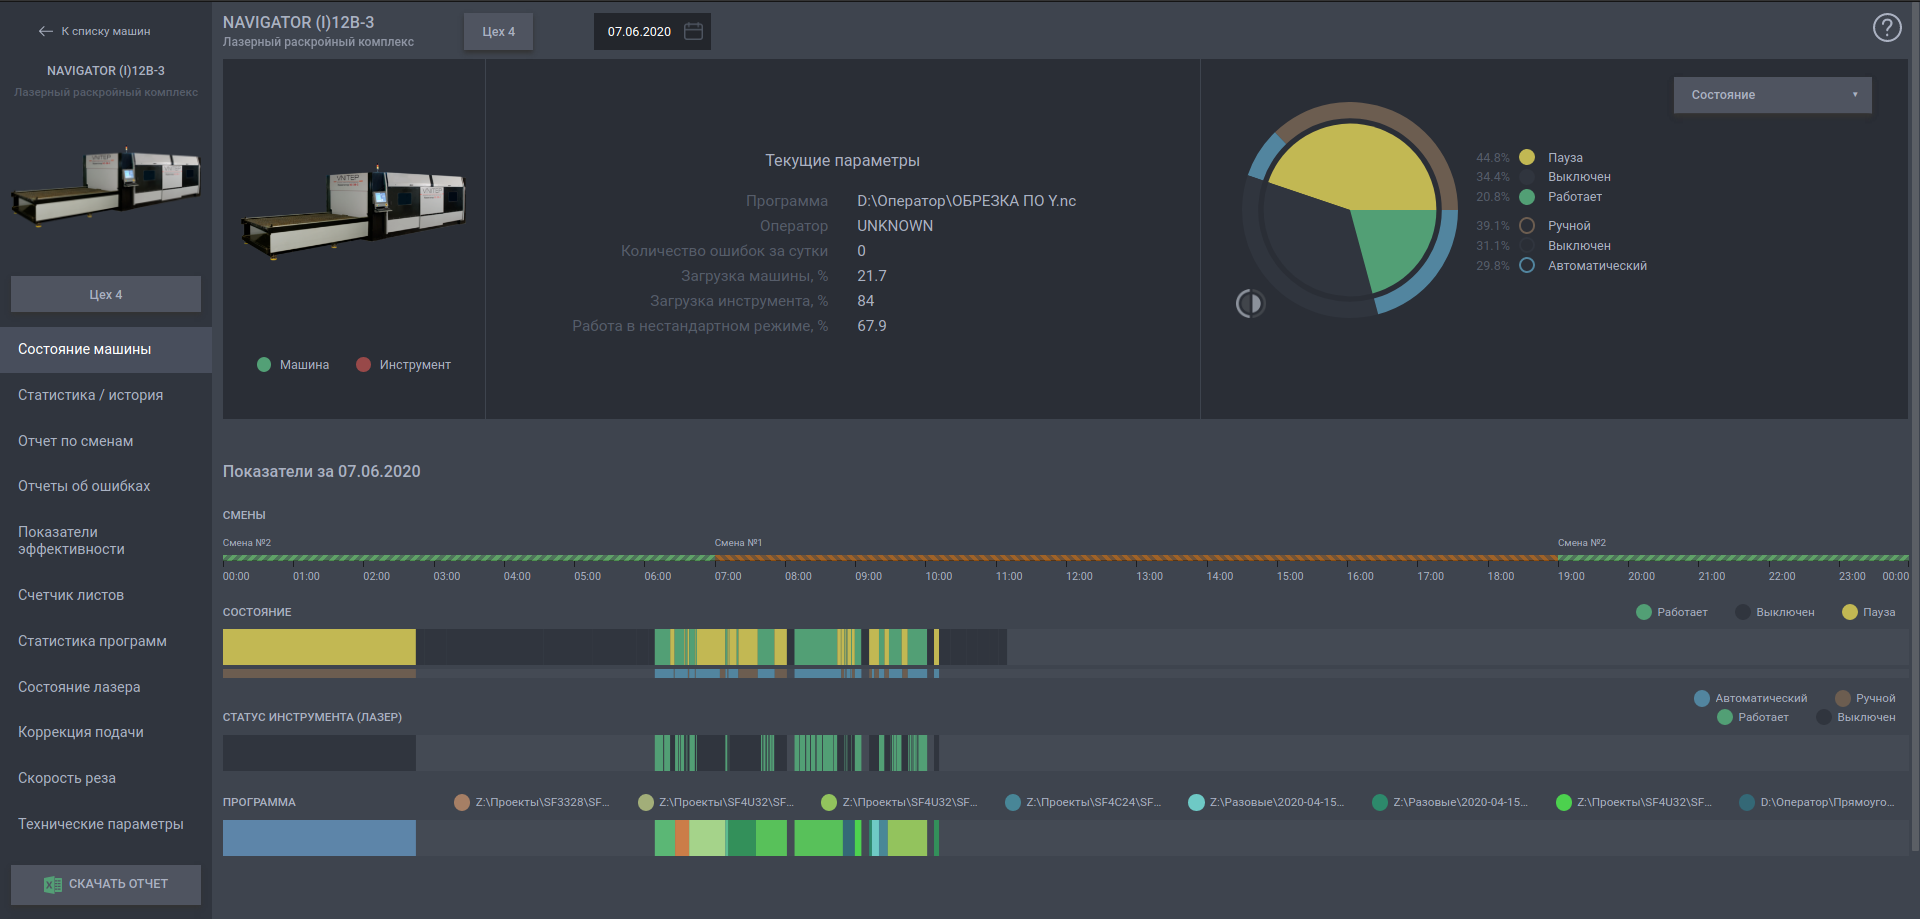
\includegraphics[width=11cm]{general.png}
\end{figure}


\end{frame}

%-------------------------------------------------------------------------------

\section{Проблема и гипотеза}

\begin{frame}
    \frametitle{\insertsection}

\textbf{Проблема:}
Отсутствие автоматизированной системы прогнозирования и выявления потенциальных неисправностей
на станках Навигатор, позволяющая сохранить ресурсы пользователей станка.

\vspace{\baselineskip}

\textbf{Гипотеза:}
Предполагается, что использование методов интеллектуального анализа данных
может помочь в решении обозначенной проблемы.


\end{frame}

%-------------------------------------------------------------------------------

\section{Анализ подходов}

\begin{frame}
\frametitle{\insertsection}

\textbf{Используемые методы и подходы в задачах прогнозирования и определения неисправностей в  различных устройствах:}
\begin{itemize}
    \item анализ временных рядов;
    \item методы машинного обучения: классификация, регрессия и кластеризация;
    \item нейронные сети различных архитектур: рекуррентные, сверточные и другие;
    \item методы теории фильтров и динамических систем: фильтры Калмана, адаптивные фильтры.
\end{itemize}

\end{frame}

%-------------------------------------------------------------------------------


\section{Входные и выходные данные}

\begin{frame}
\frametitle{\insertsection}

\textbf{Входные данные:}
\begin{itemize}
    \item температура лазера;
    \item мощность лазера;
    \item установленная мощность лазера;
    \item время в Unix формате (мировое время).
\end{itemize}

\textbf{Выходные данные:}
\begin{itemize}
    \item отчет о состоянии станка.
\end{itemize}


\end{frame}

%-------------------------------------------------------------------------------


\section{Тестирование на нормальность}

\begin{frame}
\frametitle{\insertsection}

\begin{figure}
    \center
    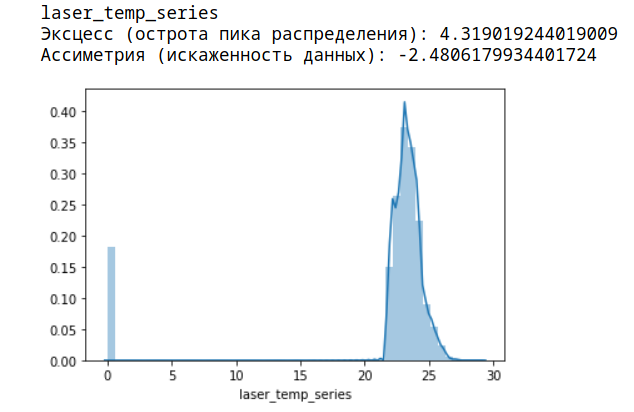
\includegraphics[width=5cm]{tempstruct.png}
    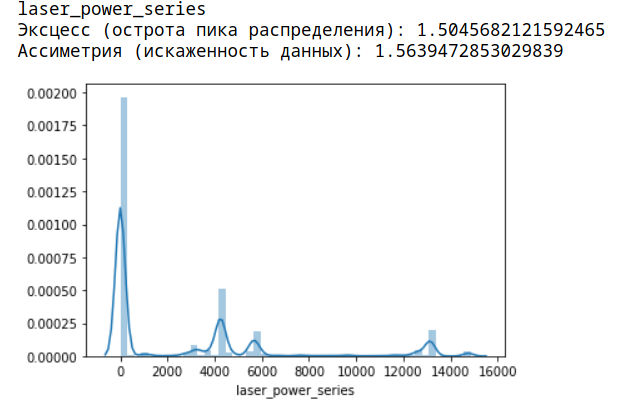
\includegraphics[width=5cm]{powerstruct.png}
\end{figure}

\begin{figure}
    \center
    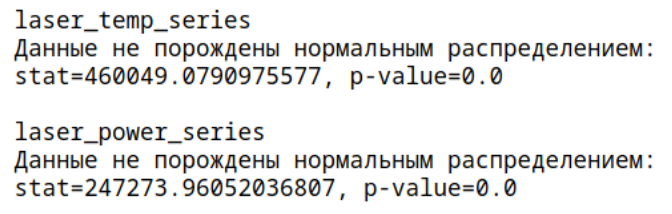
\includegraphics[width=5cm]{normaltestpart.png}
\end{figure}

\end{frame}

%-------------------------------------------------------------------------------


\section{Свойства параметров температуры и мощности}

\begin{frame}
\frametitle{\insertsection}

\begin{figure}
    \center
    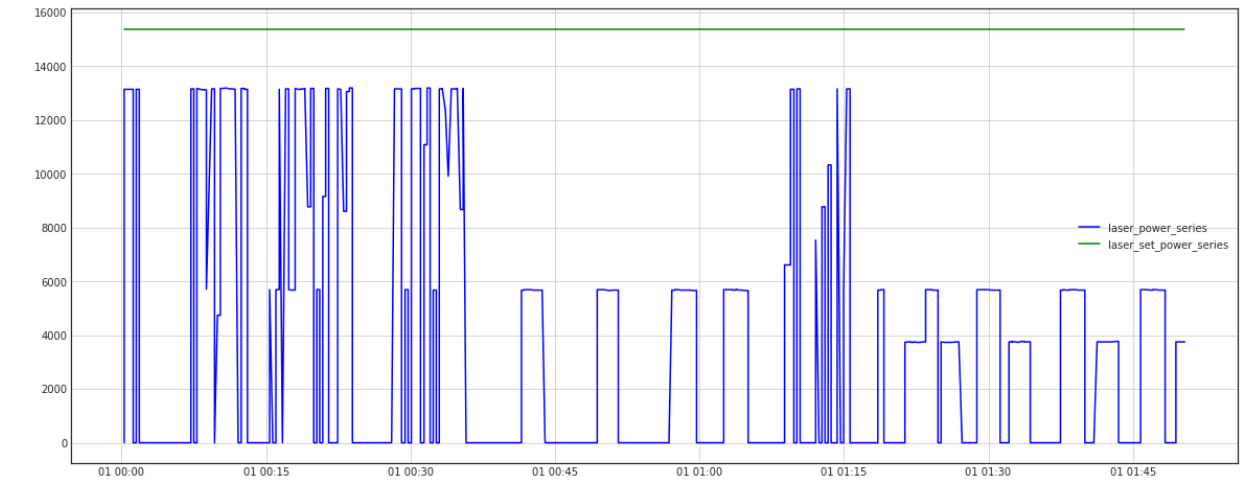
\includegraphics[width=8cm]{checkpower.png}
    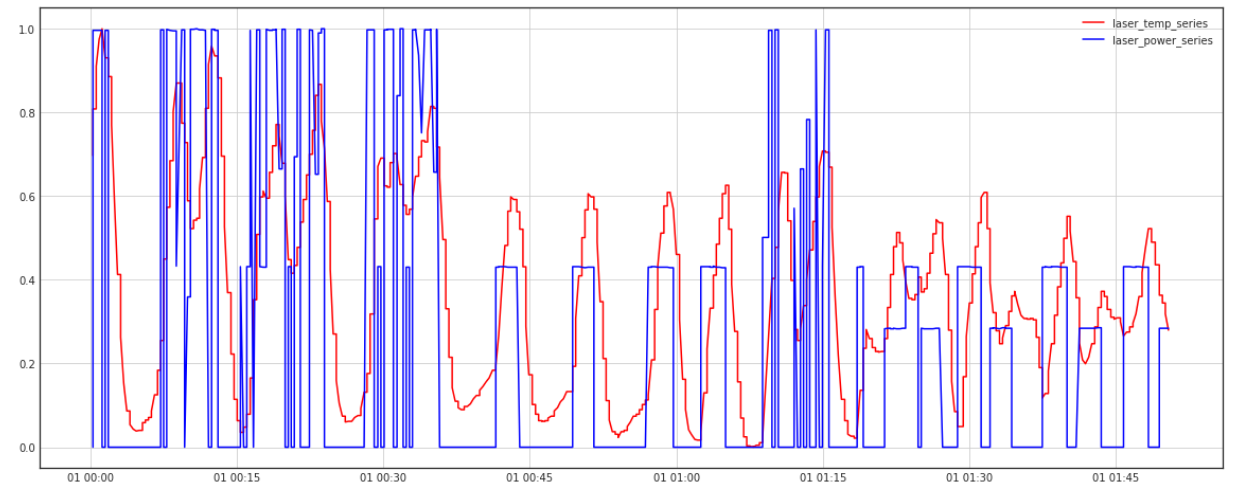
\includegraphics[width=8cm]{powertemp.png}
\end{figure}


\end{frame}

%-------------------------------------------------------------------------------


\section{Тестирование на стационарность}

\begin{frame}
\frametitle{\insertsection}

\begin{figure}
    \center
    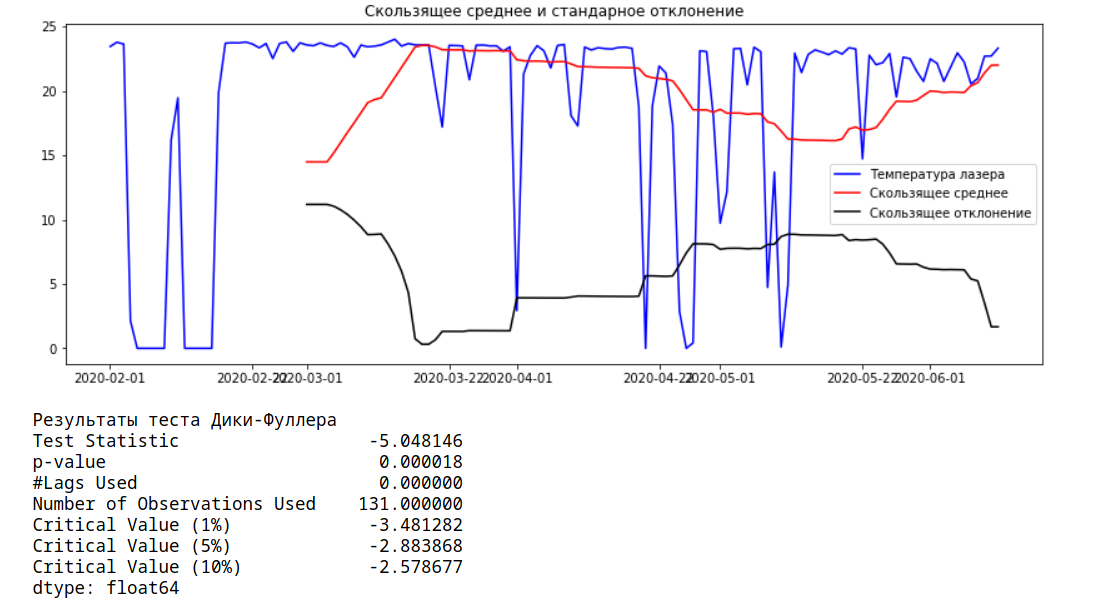
\includegraphics[width=10cm]{fullertemp.png}
\end{figure}

\end{frame}

%-------------------------------------------------------------------------------


\section{Прогнозирование на основе LSTM}

\begin{frame}
\frametitle{\insertsection}

\begin{figure}
    \center
    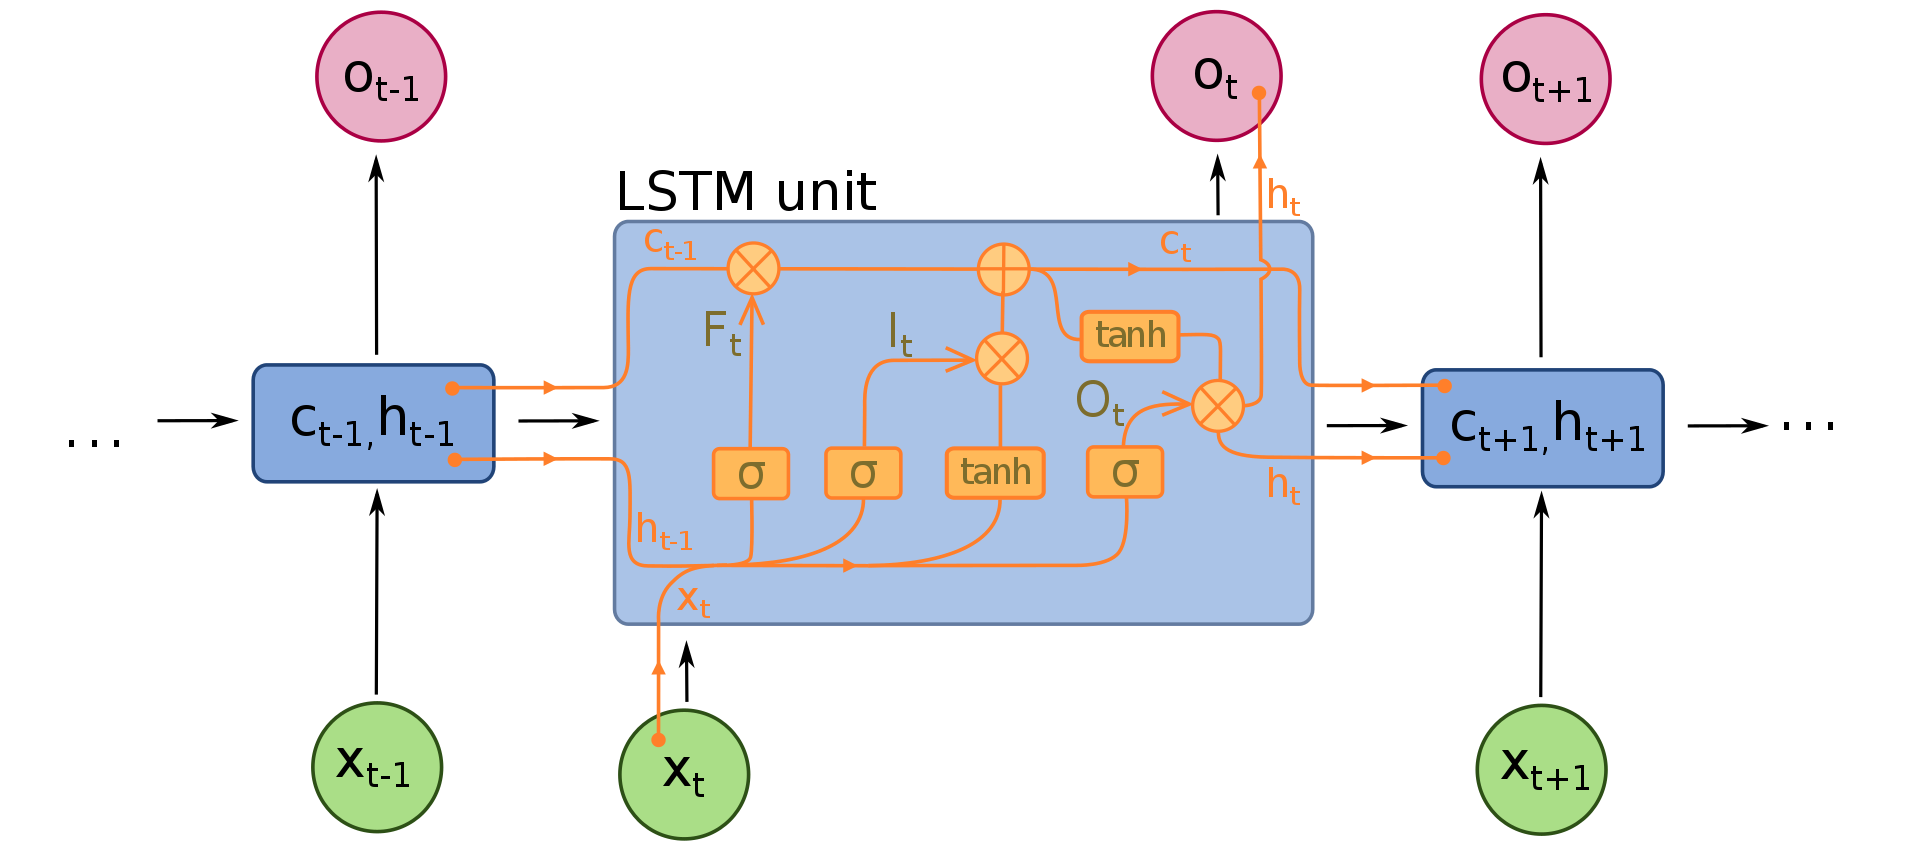
\includegraphics[width=10cm]{lstm.png}
\end{figure}


\end{frame}

%-------------------------------------------------------------------------------


\section{Оптимальные окна}

\begin{frame}
\frametitle{\insertsection}

\vspace{\baselineskip}

\begin{figure}
    \center
    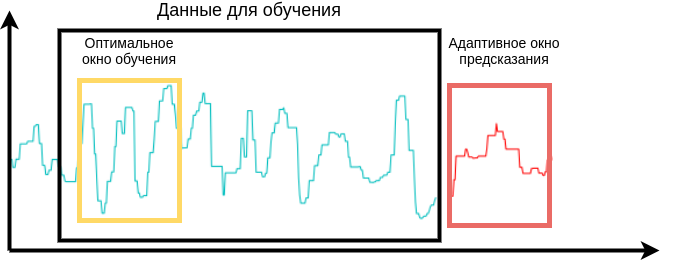
\includegraphics[width=10cm]{windows.png}
\end{figure}

\end{frame}

%-------------------------------------------------------------------------------

\section{Результаты предсказания}

\begin{frame}
\frametitle{\insertsection}

\begin{figure}
    \center
    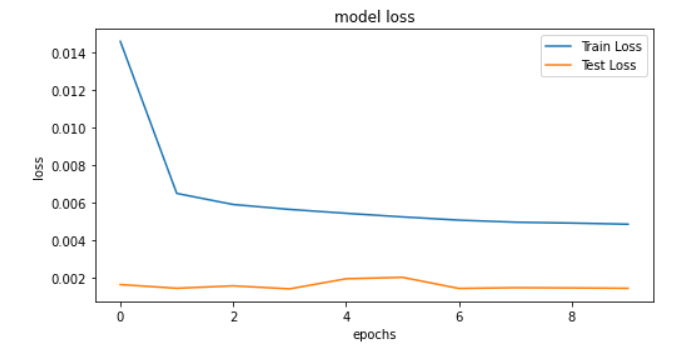
\includegraphics[width=5cm]{losstemp.png}
    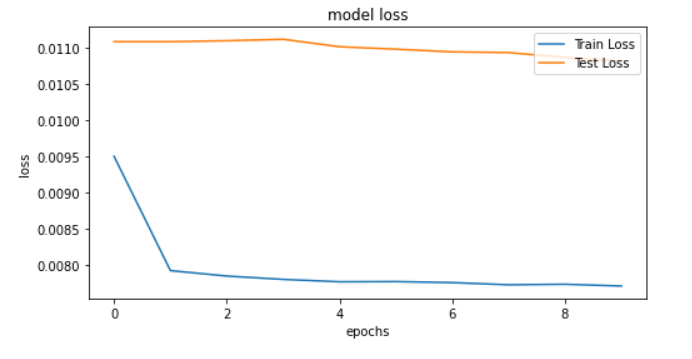
\includegraphics[width=5cm]{losspower.png}
\end{figure}

\begin{figure}
    \center
    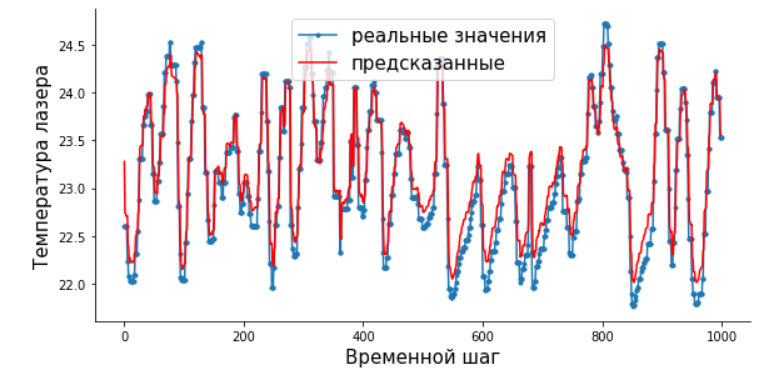
\includegraphics[width=5cm]{predtemp.png}
    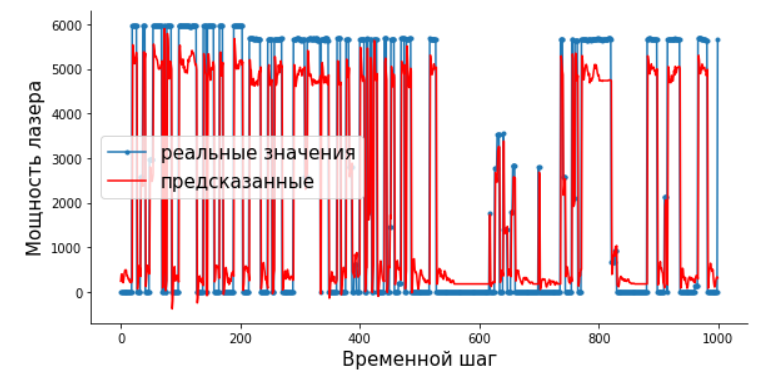
\includegraphics[width=5cm]{predpower.png}
\end{figure}


\end{frame}

%-------------------------------------------------------------------------------

\section{Кластеризация на основе алгоритма k-Shape}

\begin{frame}
\frametitle{\insertsection}

\begin{figure}
    \center
    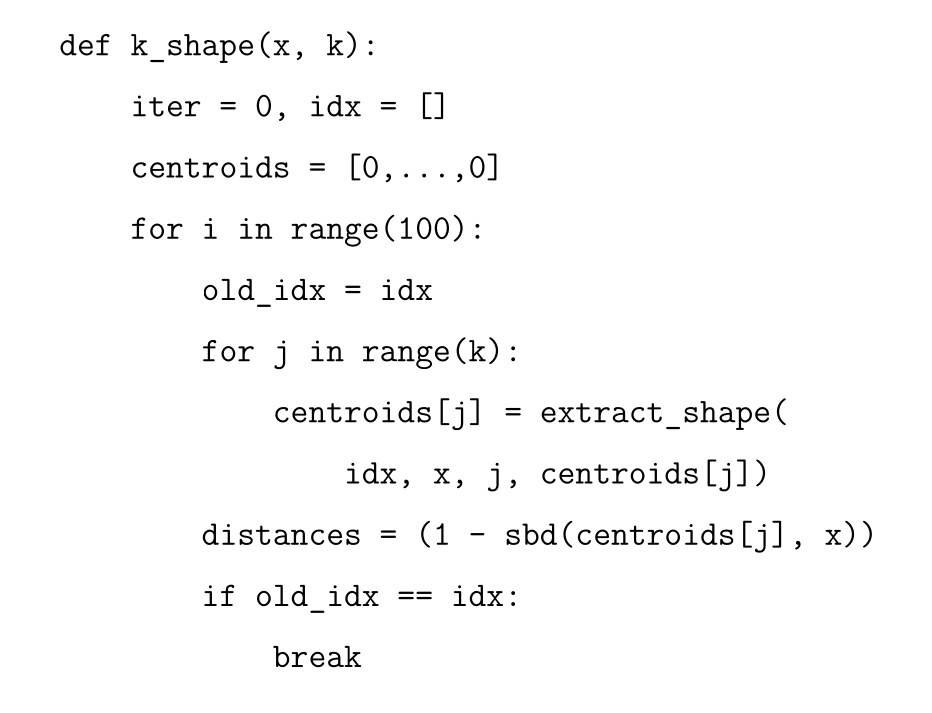
\includegraphics[width=5.5cm]{kshape.png}
    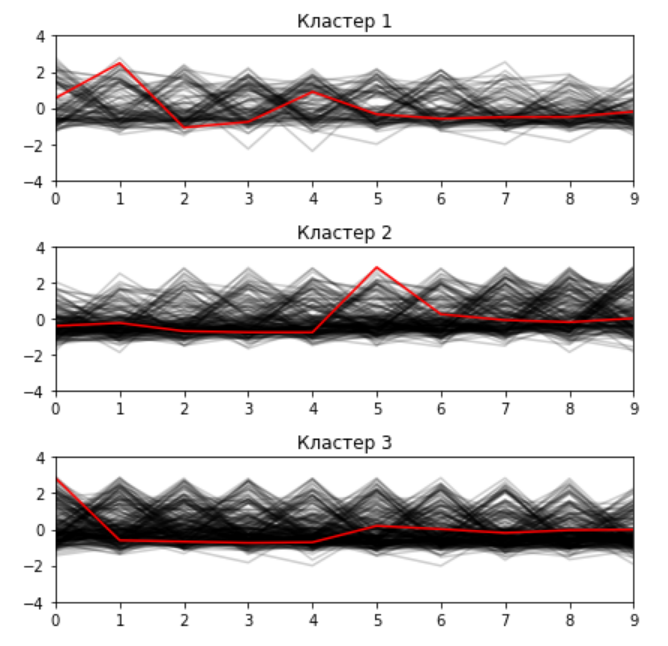
\includegraphics[width=5cm]{kshaperes.png}
\end{figure}

\begin{figure}
    \center
    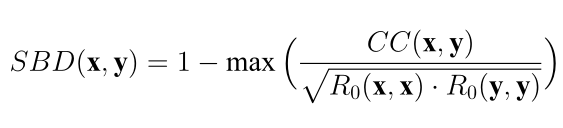
\includegraphics[width=5cm]{sbdmath.png}
\end{figure}


\end{frame}

%-------------------------------------------------------------------------------

\section{Архитектура}

\begin{frame}
\frametitle{\insertsection}

\begin{figure}
    \center
    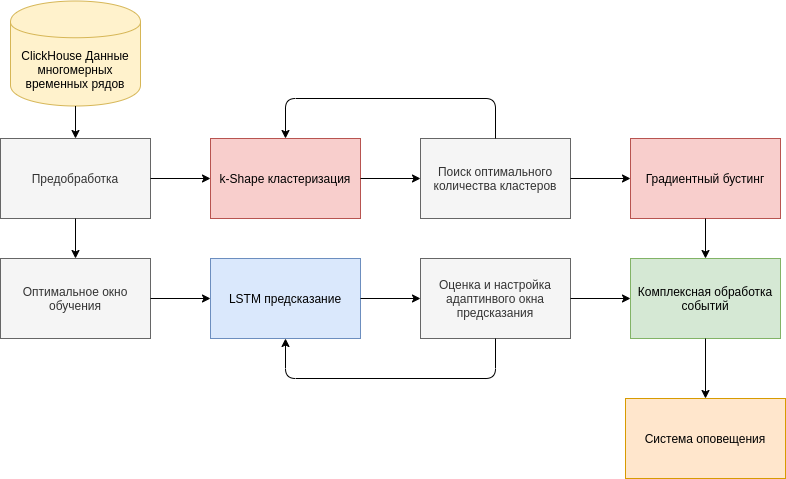
\includegraphics[width=10cm]{pipeline.png}
\end{figure}

\end{frame}

%-------------------------------------------------------------------------------

\section{Внедрение в эксплуатацию}

\begin{frame}
\frametitle{\insertsection}

\begin{figure}
    \center
    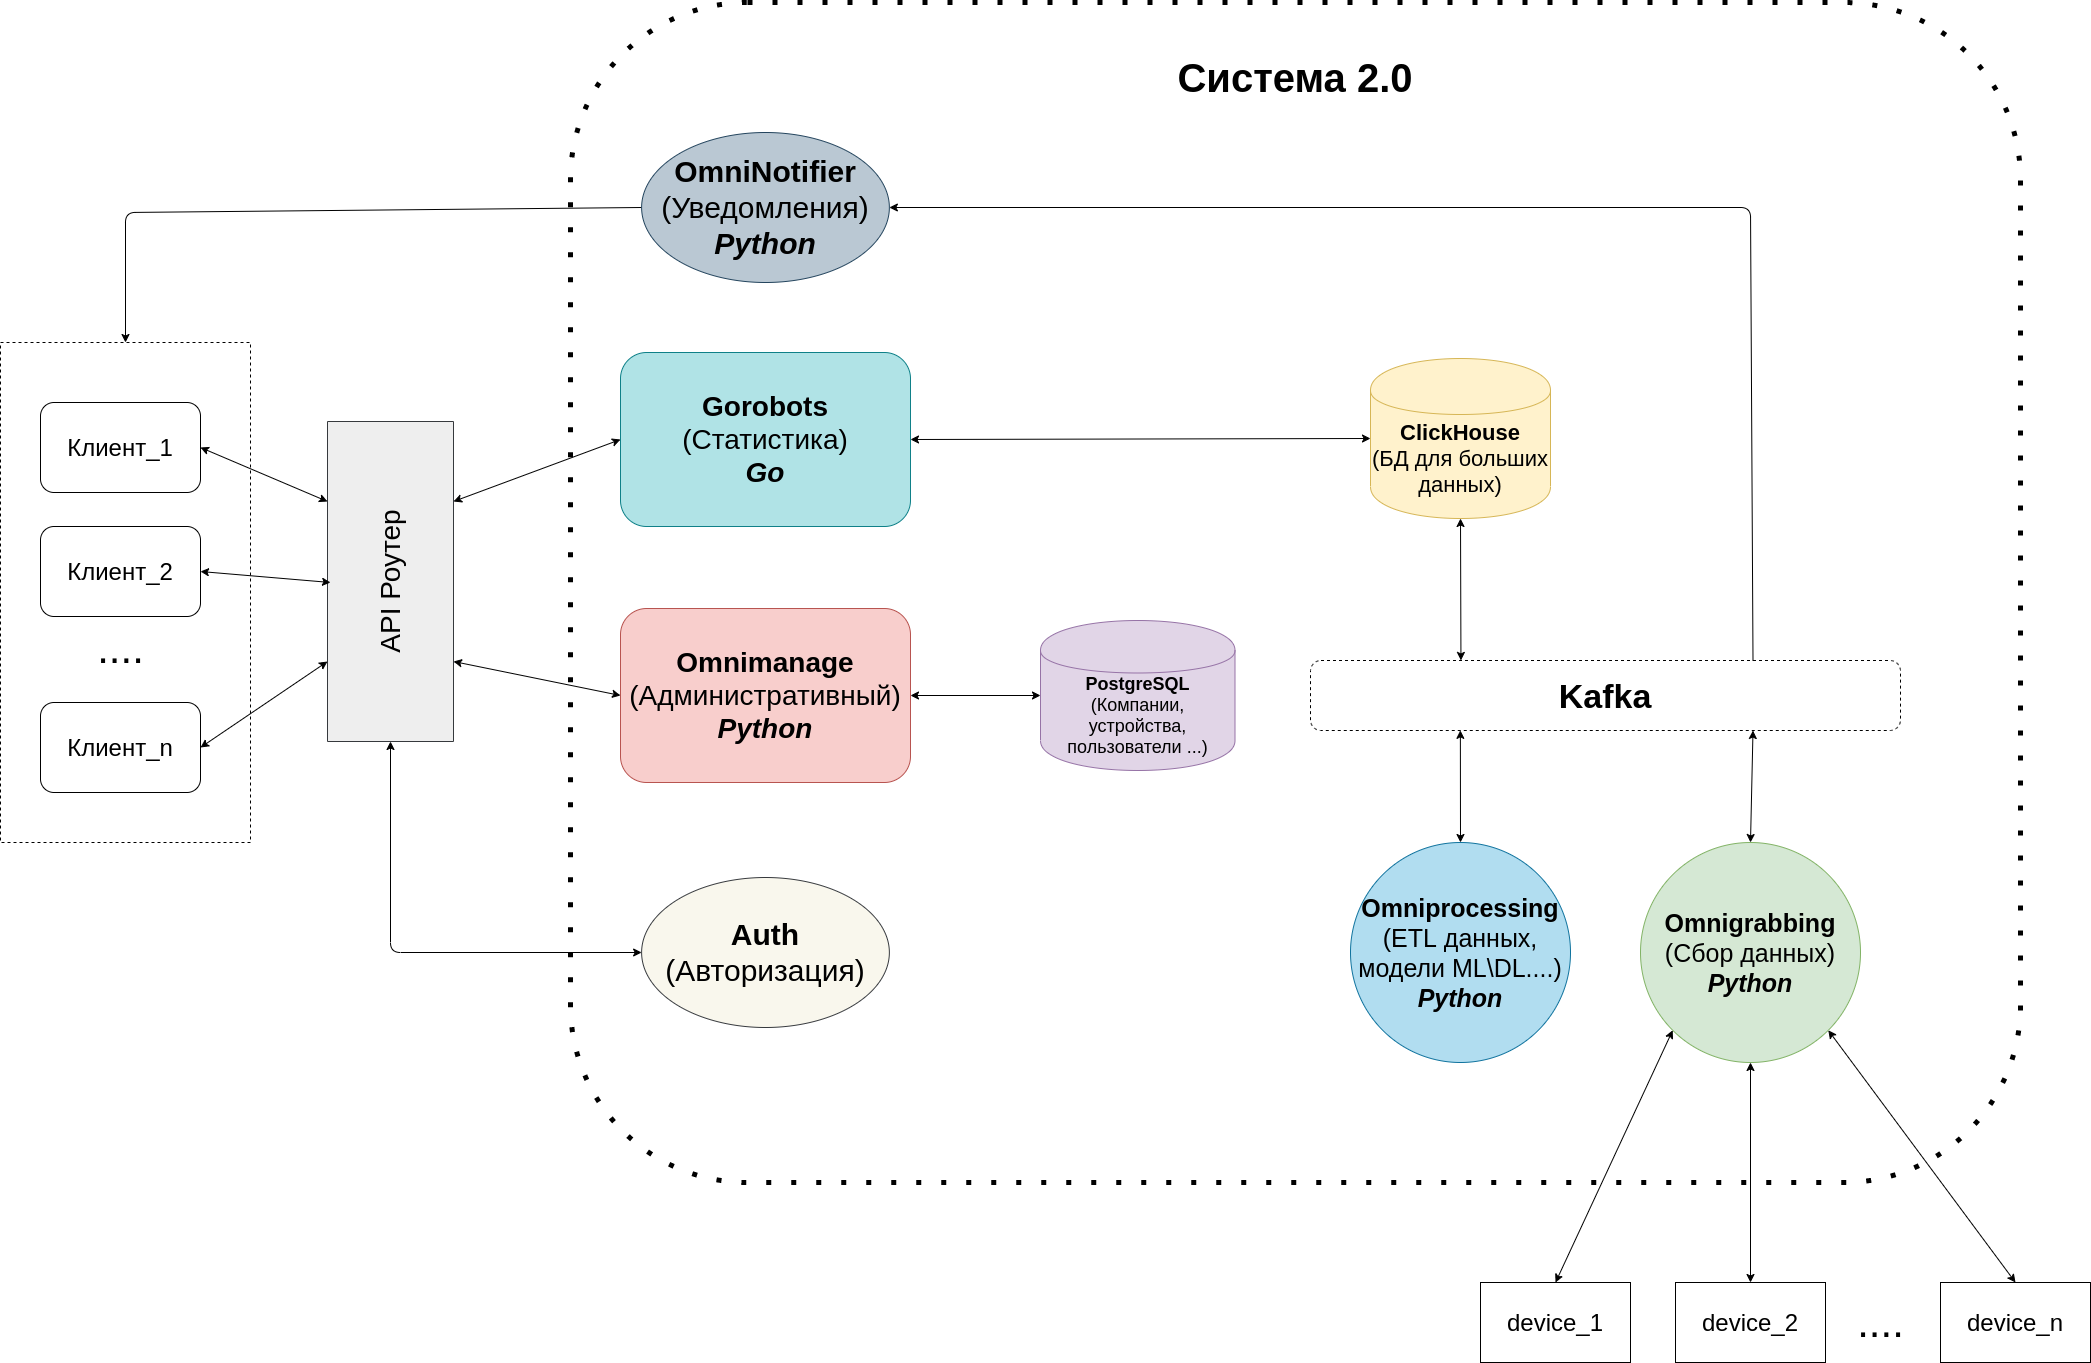
\includegraphics[width=10cm]{sys2.png}
\end{figure}


\end{frame}

%-------------------------------------------------------------------------------

\section{Заключение}

\begin{frame}

\vspace{\baselineskip}

\vspace{\baselineskip}

\begin{center}
    \Huge{\textbf{Заключение}}
\end{center}

\end{frame}

%-------------------------------------------------------------------------------
